% -------------------------------------------------------------------------------------------------
%      MDSG Latex Framework
%      ============================================================================================
%      File:                  introduction-[UTF8,ISO8859-1].tex
%      Author(s):             Michael Duerr
%      Version:               1
%      Creation Date:         30. Mai 2010
%      Creation Date:         30. Mai 2010
%
%      Notes:                 - Example chapter
% -------------------------------------------------------------------------------------------------
%
\chapter{Concept}\label{sec:Concept}
- What is your plan? \\
- How do you proof that it worked? -> Metric and Experiments


\section{Coloring Environment}\label{env}
\marginpar{origin and intro}
% Introduce Gridworld, Agent actions, goal etc.
A RL environment is a versatile and unbiased instance, that can can be used to visualize agent behavior and environmental changes.
% Although a human visualization is optional, agents need to have some sort of understanding what state they are acting in. 
In figure \ref{fig:env}, the environment used in this work is presented. It originated from an openAI project called ``Minimalistic Gridworld Environment'' \cite{chwi18}, which is designed for one agent whose main goal is to solve labyrinth puzzles. For the purpose of this research however, the environment is changed heavily, becoming the ``Coloring Environment''. Multiple agents can act in it with a new goal - to color all walkable cells.

\begin{figure}[hpbt]
    \centering
    %%----start of first subfigure----
    \subfloat[Human visualization of the coloring environment. A dot represents one agent. Cells change their color when agents moves  on them.]{
        \label{fig:env} %% label for first subfigure
        \includegraphics[width=0.35\linewidth]{pictures/Gridworld}}
    \hspace{0.01\textwidth}
    %%----start of second subfigure----
    \subfloat[Simplified agent observation of the current environment state. The number 1 represents a colored cell.]{
        \label{fig:bin_env} %% label for second subfigure
        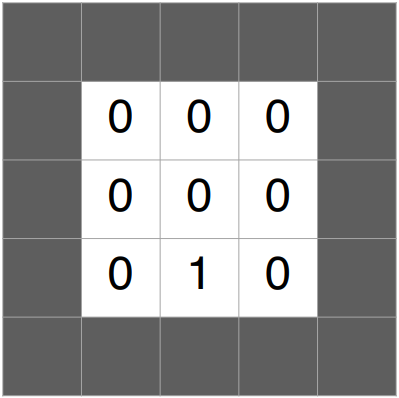
\includegraphics[width=0.35\linewidth]{pictures/binary_gridworld}}
    \caption[Coloring Environment]{Representations of the coloring environment}
    \label{fig:multipic_env} %% label for entire figure
\end{figure}

\marginpar{cell objects}
Figure \ref{fig:bin_env} shows a simplified environment observation an agent processes each timestep. Every environment cell holds information about the object it represents, being either Walls, Floors or Agents. Each object contains information about its current color, whether or not it is accessible for an agent and, in case of a floor tile, if it is colored.

\marginpar{cell objects}
Floor cells keep the coloration state in binary form, as displayed in \ref{fig:bin_env}, with a 1 signalizing that the cell is colored. The environment reacts to agents movements by coloring the cells they visit. Agents successfully solve the environment once all fields are colored. Otherwise agents loose by using up a limited amount of steps. If a cell is already in coloration state 1 and an agent walks over it again the bit is switched and the cell is reset to 0, removing its coloration. Besides moving up, down, left and right an agent can also execute the action wait.

\marginpar{cooperative multiagents}
When multiple agents act in the coloring environment each one has a different color. In the human representation (figure \ref{fig:env}) cells adopt the color of the capturing agents. The primary focus in cooperative agent compositions is only the binary state. All agents receive the same maximum reward when the grid is fully colored, making it irrelevant what colors the cells have.

\marginpar{mixed-motive multiagents}
The opposite is the case in competitive scenarios. In mixed-motive settings for example, agents only gain high rewards once the grid is fully colored, with the twists that it depends on their contribution. The reward is generated by looking up the percentage a color is present and assigning that value as reward to the corresponding agent. In a fully competitive scenario the reward calculations stay the same only disabling the bit switching. Therefore, agents can capture already colored cells when they walk over them, dying them in their color.

\section{Market Settings}
\marginpar{MARL Challenges}
Each of the three compositions presented in chapter \ref{env} lead to learning problems or game losses. Cooperation may reward misbehavior, namely field resetting, leading to the CAP of chapter \ref{CAP}. In mixed-motive or fully competitive settings the overall goal may be never reached due to greediness or disorder. This research further compares the effects of markets not only on competitive settings as suggested by Schmid et al. \cite{scbe21}, but rather on all three configurations.

\marginpar{action space}
As mentioned earlier, agents have five possible action choices each timestep: moving up, down, left, right or simply to wait. Adding a market to the stochastic game expands this one dimensional action space into a three dimensional action space. 
- am

- am-goal

- am-goal-no-reset

- sm

- sm-goal

- sm-goal-no-reset